\section{Introduction}

L’ordonnancement des processus est une composante essentielle des systèmes d’exploitation, car il détermine la manière dont les processus se partagent le processeur. Selon la politique choisie, l’objectif peut être de maximiser l’efficacité, d’assurer une certaine équité ou encore de réduire le temps d’attente des tâches.

Les listes chaînées sont des structures qui permettent de stocker et de manipuler facilement des processus, que ce soit sous la forme d’une file FIFO, d’une pile LIFO, d’une liste triée, ou encore d’autres types de structures.

La première politique étudiée est le FCFS (First Come, First Served), où les processus sont exécutés dans l’ordre d’arrivée. Pour la simuler, une file FIFO est utilisée, permettant d’ajouter les processus à la fin de la file et de les retirer au début. La seconde politique est le SJF (Shortest Job First), où les processus les plus courts sont traités en priorité. Dans ce cas, une liste triée est utilisée afin d’insérer chaque processus à la position correcte, garantissant que les durées restent classées dans l’ordre croissant.

L’objectif de ce TP est ainsi de comprendre le fonctionnement et la manipulation des listes chaînées tout en observant l’impact concret de chaque politique sur l’exécution des processus.

\newpage

\section{First Come, First Served}
\subsection{Introduction}

L’ordonnancement FCFS (First Come, First Served) exécute les processus selon leur ordre d’arrivée. Ceux-ci sont stockés dans une file d’attente de type FIFO (First In, First Out), où le premier processus inséré est également le premier retiré.
L’implémentation utilise cette structure pour gérer simplement la succession des exécutions. Chaque processus terminé libère la place au suivant dans la file.
Ci dessous un schéma représentant la file FIFO (cf. Figure~\ref{fig:fcfs_fifo}).
\begin{figure}[H]
    \centering
    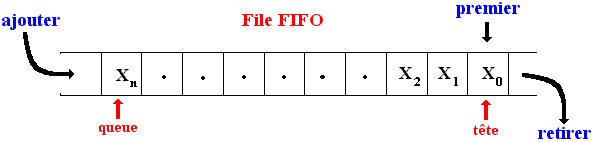
\includegraphics[width=8cm]{../images/fifo.png}
    \caption{Structure de la file FIFO pour FCFS}
    \label{fig:fcfs_fifo}
\end{figure}

\subsection{Résultats et analyse}

Après avoir implémenté la politique FCFS à l'aide d'une file FIFO, nous avons observé les résultats suivants :
De plus, nous avons analysé les performances de cette politique en termes de compléxité. Ici pour notre algorithme FCFS, la compléxité est de O(n) car chaque processus doit être ajouté et retiré de la file une seule fois.

%%%%%%%%%%%%%%%%%%%%%%%%%%%%%%%%
\newpage
%%%%%%%%%%%%%%%%%%%%%%%%%%%%%%%%


\section{Shortest Job First}
\subsection{Introduction}
L’ordonnancement SJF (Shortest Job First) exécute en priorité les processus dont la durée d’exécution est la plus courte. Les processus sont organisés dans une liste triée en fonction de leur temps d’exécution, ce qui permet de sélectionner en premier celui dont la charge est minimale.
L’implémentation repose sur cette structure ordonnée qui facilite la recherche du processus le plus court à chaque étape. Une fois un processus terminé, le suivant le plus court est choisi automatiquement.
Ci-dessous (cf. Figure~\ref{fig:lst_trie}) un schéma illustrant la liste triée utilisée pour cet ordonnancement.
\begin{figure}[H]
    \centering
    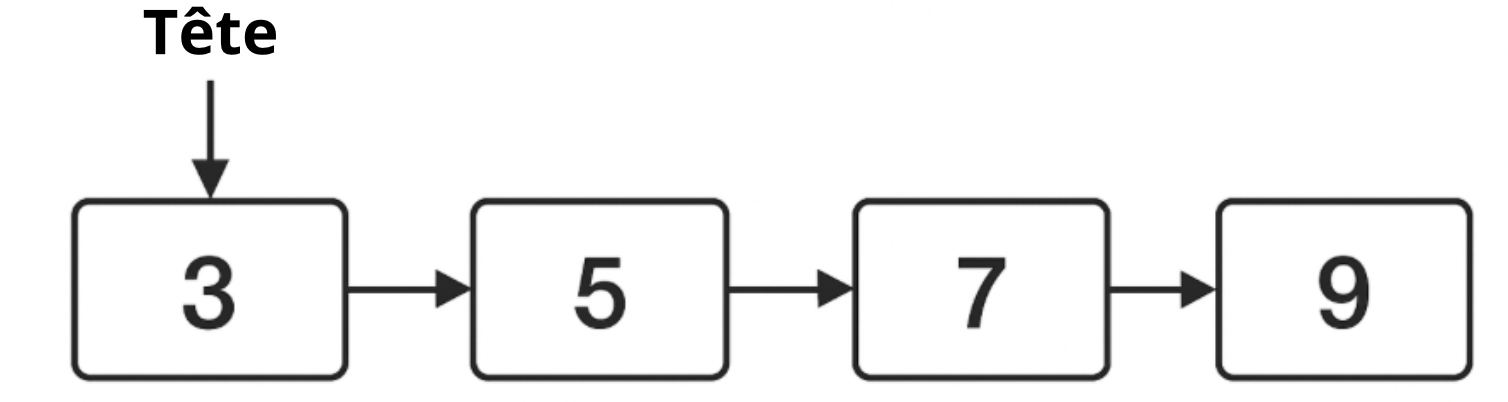
\includegraphics[width=8cm]{../images/lst_trie.png}
    \caption{Structure de la file FIFO pour FCFS}
    \label{fig:lst_trie}
\end{figure}

\subsection{Résultats et analyse}

%%%%%%%%%%%%%%%%%%%%%%%%%%%%%%%%
\newpage
%%%%%%%%%%%%%%%%%%%%%%%%%%%%%%%%

\section{Conclusion}

Dans ce TP, nous avons 